\documentclass[a4paper,10pt]{article}

\usepackage[ansinew]{inputenc}
\usepackage[spanish]{babel}
\usepackage{graphicx}
\usepackage{listings}
\usepackage{appendix}
\usepackage{pdfpages}
\usepackage{fancyhdr}
\usepackage{ulem}
\usepackage{float}
\pagestyle{fancy}

\def\dashuline{\bgroup 
  \ifdim\ULdepth=\maxdimen  % Set depth based on font, if not set already
   \settodepth\ULdepth{(j}\advance\ULdepth.4pt\fi
  \markoverwith{\kern.15em
  \vtop{\kern\ULdepth \hrule width .3em}%
  \kern.15em}\ULon}

\begin{document}

\lhead{\fancyplain{}{Base de Datos 75.15}}
\rhead{\fancyplain{}{Trabajo Pr\'actico Grupal}}

\setcounter{page}{2}

\newpage
\thispagestyle{empty}
\tableofcontents

\newpage
\section{Modelo Entidad Relaci\'on}
  \subsection{Diagrama}
    \begin{center}
      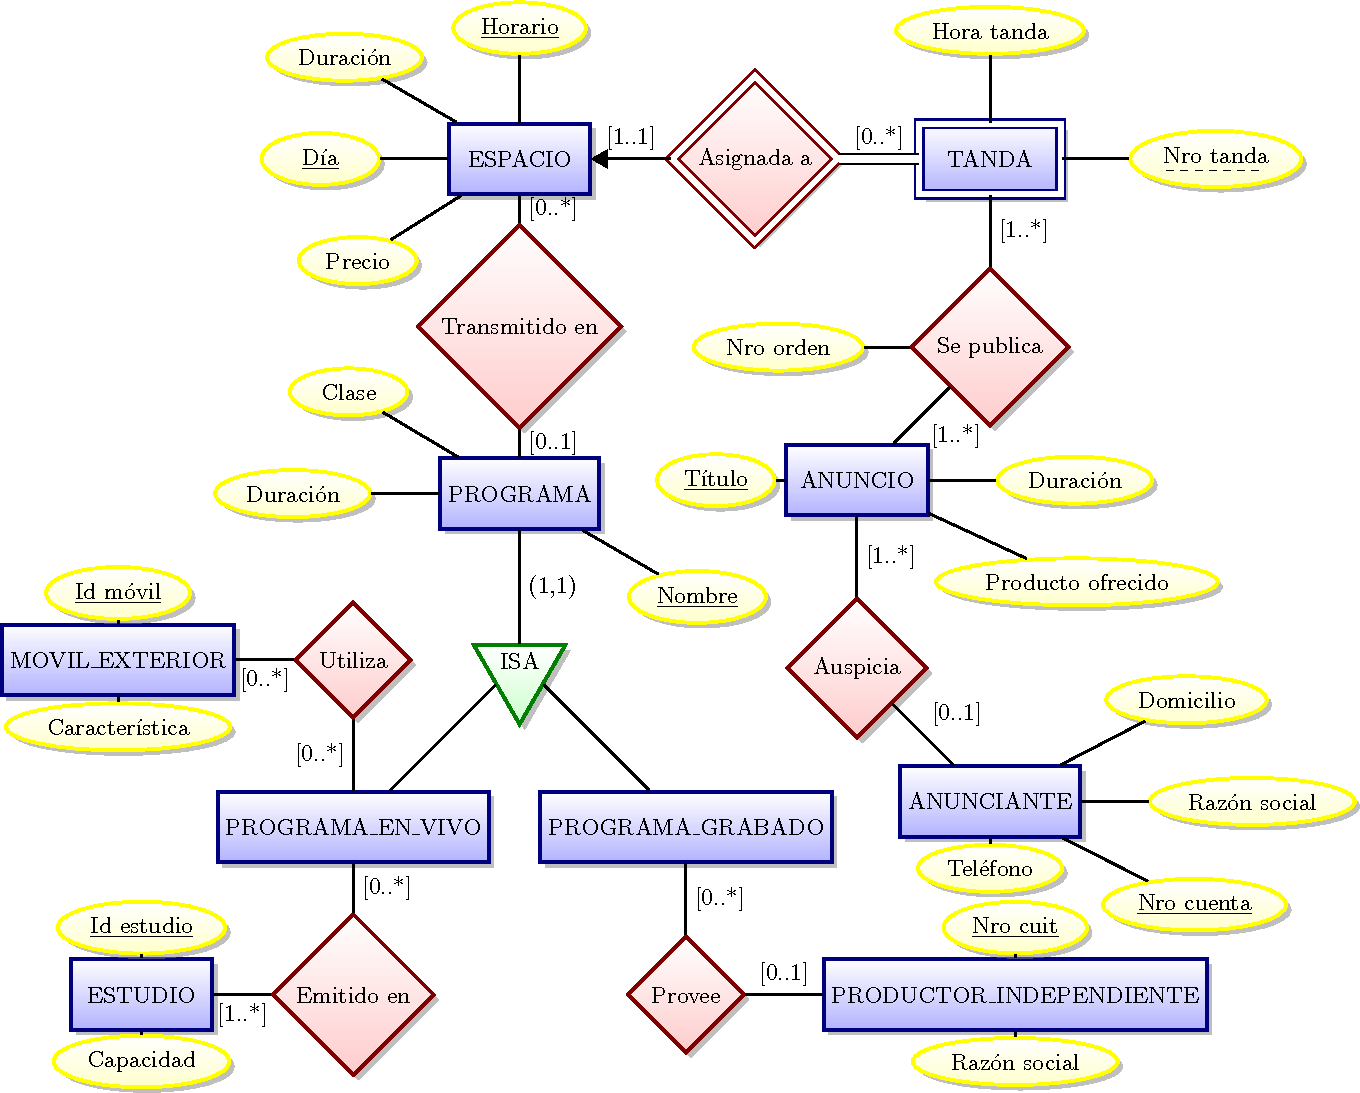
\includegraphics[width=18cm, height=12cm, angle=-90]{ModeloE-R/ModeloE-R.png}   
    \end{center}
  \subsection{Hip\'otesis}
    \begin{enumerate}
      \item Cada m\'ovil de exterior posee un id que lo identifica un\'ivocamente. 
      \item Un programa puede ser en vivo o grabado.
      \item S\'olo los programas en vivo poseen estudios de emisi\'on.
    \end{enumerate}
    
  \subsection{Diccionario}
    \subsubsection{Entidades}
    \begin{flushleft}
      \begin{large} \bf{Espacio} \end{large}
    \end{flushleft}
      \begin{tabular}{| p{2cm} | p{9cm} |}
	\hline
	\multicolumn{2}{|l|}{\bf{Descripci\'on:}} \\
	\hline
	\multicolumn{2}{|l|}{Un espacio es una divisi\'on del horario de transmisi\'on del canal.} \\
	\hline	
	\multicolumn{2}{|l|}{\bf{Especificaci\'on de atributos:}} \\
	\hline
	- D\'ia & El d\'ia en el que se emite el espacio. \\
	\hline \hline
	- Horario & El horario en el que se emite el espacio. \\
	\hline \hline
	- Duraci\'on & La duraci\'on del espacio.\\
	\hline \hline
	- Precio & El precio por segundo en el aire del espacio.\\
	\hline
	\multicolumn{2}{|l|}{\bf{Especificaci\'on de identificador \'unico:}} \\
	\hline
	\multicolumn{2}{|l|}{- D\'ia + Horario} \\
	\hline
      \end{tabular}
    
    \begin{flushleft}
      \begin{large} \bf{Tanda} \end{large}
    \end{flushleft}
      \begin{tabular}{| p{2cm} | p{9cm} |}
	\hline
	\multicolumn{2}{|l|}{\bf{Descripci\'on:}} \\
	\hline
	\multicolumn{2}{|l|}{Un tanda es un espacio donde se publicitan anuncios.} \\
	\hline	
	\multicolumn{2}{|l|}{\bf{Especificaci\'on de atributos:}} \\
	\hline
	- Hora\_tanda & La hora de comienzo de la tanda. \\
	\hline \hline
	- Nro\_tanda & El n\'umero de tanda correspondiente a un programa. \\
	\hline
	\multicolumn{2}{|l|}{\bf{Especificaci\'on de identificador \'unico:}} \\
	\hline
	\multicolumn{2}{|l|}{- D\'ia + Horario + Nro\_tanda} \\
	\hline
      \end{tabular}

    \begin{flushleft}
      \begin{large} \bf{Anuncio} \end{large}
    \end{flushleft}
      \begin{tabular}{| p{2cm} | p{9cm} |}
	\hline
	\multicolumn{2}{|l|}{\bf{Descripci\'on:}} \\
	\hline
	\multicolumn{2}{|l|}{Un anuncio es un espacio, dentro de una tanda, destinado a dar a conocer} \\
	\multicolumn{2}{|l|}{un producto.} \\
	\hline	
	\hline	
	\multicolumn{2}{|l|}{\bf{Especificaci\'on de atributos:}} \\
	\hline
	- T\'itulo & El t\'itulo del anuncio. \\
	\hline \hline
	- Duraci\'on & La duraci\'on del anuncio. \\
	\hline \hline
	- Producto \newline ofrecido & El producto ofrendido del anuncio. \\
	\hline
	\multicolumn{2}{|l|}{\bf{Especificaci\'on de identificador \'unico:}} \\
	\hline
	\multicolumn{2}{|l|}{- T\'itulo} \\
	\hline
      \end{tabular}

    \newpage
    \begin{flushleft}
      \begin{large} \bf{Anunciante} \end{large}
    \end{flushleft}
      \begin{tabular}{| p{2cm} | p{9cm} |}
	\hline
	\multicolumn{2}{|l|}{\bf{Descripci\'on:}} \\
	\hline
	\multicolumn{2}{|l|}{Un anunciante auspicia a lo sumo un producto, mediante un anuncio.} \\
	\hline	
	\multicolumn{2}{|l|}{\bf{Especificaci\'on de atributos:}} \\
	\hline
	- Nro\_cuenta & El n\'umero de cuenta del anunciante. \\
	\hline \hline
	- Domicilio & El domicilio del anunciante. \\
	\hline \hline
	- Raz\'on\_ \newline social & La raz\'on social del anunciante. \\
	\hline \hline
	- Tel\'efono & El tel\'efono del anunciate. \\
	\hline
	\multicolumn{2}{|l|}{\bf{Especificaci\'on de identificador \'unico:}} \\
	\hline
	\multicolumn{2}{|l|}{- Nro\_cuenta} \\
	\hline
      \end{tabular}

    \begin{flushleft}
      \begin{large} \bf{Programa} \end{large}
    \end{flushleft}
      \begin{tabular}{| p{2cm} | p{9cm} |}
	\hline
	\multicolumn{2}{|l|}{\bf{Descripci\'on:}} \\
	\hline
	\multicolumn{2}{|l|}{Un programa es un bloque con contenido que transmitir\'a el canal} \\
	\multicolumn{2}{|l|}{periodicamente} \\
	\hline	
	\multicolumn{2}{|l|}{\bf{Especificaci\'on de atributos:}} \\
	\hline
	- Clase & El tipo de programa que se transmite. \\
	\hline \hline
	- Nombre & Nombre del programa. \\
	\hline \hline
	- Duraci\'on & La duraci\'on del programa.\\
	\hline
	\multicolumn{2}{|l|}{\bf{Especificaci\'on de identificador \'unico:}} \\
	\hline
	\multicolumn{2}{|l|}{- Nombre} \\
	\hline
      \end{tabular}
  
    \begin{flushleft}
      \begin{large} \bf{Programa\_en\_vivo} \end{large}
    \end{flushleft}
      \begin{tabular}{| p{2cm} | p{9cm} |}
	\hline
	\multicolumn{2}{|l|}{\bf{Descripci\'on:}} \\
	\hline
	\multicolumn{2}{|l|}{Un programa en vivo es un programa que se transmite en vivo} \\
	\hline	
	\multicolumn{2}{|l|}{\bf{Especificaci\'on de atributos:}} \\
	\hline
	- No tiene & \\
	\hline
	\multicolumn{2}{|l|}{\bf{Especificaci\'on de identificador \'unico:}} \\
	\hline
	\multicolumn{2}{|l|}{- Hereda la clave de la entidad Programa} \\
	\hline
      \end{tabular} 
  
    \begin{flushleft}
      \begin{large} \bf{Programa\_grabado} \end{large}
    \end{flushleft}
      \begin{tabular}{| p{2cm} | p{9cm} |}
	\hline
	\multicolumn{2}{|l|}{\bf{Descripci\'on:}} \\
	\hline
	\multicolumn{2}{|l|}{Un programa grabado es un programa que se graba y luego se transmite} \\
	\hline	
	\multicolumn{2}{|l|}{\bf{Especificaci\'on de atributos:}} \\
	\hline
	- No tiene & \\
	\hline
	\multicolumn{2}{|l|}{\bf{Especificaci\'on de identificador \'unico:}} \\
	\hline
	\multicolumn{2}{|l|}{- Hereda la clave de la entidad Programa} \\
	\hline
      \end{tabular}

    \newpage
    \begin{flushleft}
      \begin{large} \bf{M\'ovil\_Exterior} \end{large}
    \end{flushleft}
      \begin{tabular}{| p{2cm} | p{9cm} |}
	\hline
	\multicolumn{2}{|l|}{\bf{Descripci\'on:}} \\
	\hline
	\multicolumn{2}{|l|}{Un m\'ovil exterior es un veh\'iculo preparado para usar en la calle durante} \\
	\multicolumn{2}{|l|}{la emisi\'on de programas en vivo} \\	
	\hline	
	\multicolumn{2}{|l|}{\bf{Especificaci\'on de atributos:}} \\
	\hline
	- Id\_movil & Identifica el movil. \\
	\hline \hline
	- Carac- \newline ter\'istica & Descripci\'on de las caracter\'isticas del movil. \\
	\hline
	\multicolumn{2}{|l|}{\bf{Especificaci\'on de identificador \'unico:}} \\
	\hline
	\multicolumn{2}{|l|}{- Id\_m\'ovil} \\
	\hline
      \end{tabular}
      
    \begin{flushleft}
      \begin{large} \bf{Estudio} \end{large}
    \end{flushleft}
      \begin{tabular}{| p{2cm} | p{9cm} |}
	\hline
	\multicolumn{2}{|l|}{\bf{Descripci\'on:}} \\
	\hline
	\multicolumn{2}{|l|}{Un estudio es el lugar donde se toma lugar un programa en vivo} \\
	\hline	
	\multicolumn{2}{|l|}{\bf{Especificaci\'on de atributos:}} \\
	\hline
	- Id\_estudio & Identifica el estudio. \\
	\hline \hline
	- Capacidad & Cantidad de personas que entran en el estudio. \\
	\hline
	\multicolumn{2}{|l|}{\bf{Especificaci\'on de identificador \'unico:}} \\
	\hline
	\multicolumn{2}{|l|}{- Id\_estudio} \\
	\hline
      \end{tabular} 
      
    \begin{flushleft}
      \begin{large} \bf{Productor\_independiente} \end{large}
    \end{flushleft}
      \begin{tabular}{| p{2cm} | p{9cm} |}
	\hline
	\multicolumn{2}{|l|}{\bf{Descripci\'on:}} \\
	\hline
	\multicolumn{2}{|l|}{Un productor independiente es aquel que se graba un programa y lo} \\
	\multicolumn{2}{|l|}{entrega al canal para ser transmitido} \\	
	\hline	
	\multicolumn{2}{|l|}{\bf{Especificaci\'on de atributos:}} \\
	\hline
	- Nro\_cuit & N\'umero de CUIT del productor. \\
	\hline \hline
	- Raz\'on\_ \newline social & Raz\'on social del productor\\
	\hline
	\multicolumn{2}{|l|}{\bf{Especificaci\'on de identificador \'unico:}} \\
	\hline
	\multicolumn{2}{|l|}{- Nro\_cuit} \\
	\hline
      \end{tabular} 
   
   
    \subsubsection{Interrelaciones}
    
    \begin{flushleft}
      \begin{large} \bf{Asignada\_a} \end{large}
    \end{flushleft}
      \begin{tabular}{| p{11.4cm} |}
	\hline
	\bf{Descripci\'on:} \\
	\hline
	Las tandas son asignadas a los espacios en una programaci\'on. Un espacio puede tener asignadas muchas tandas. \\	
	\hline	
	\bf{Especificaci\'on de identificador \'unico:} \\
	\hline
	- D\'ia + Horario + Nro\_tanda \\
	\hline
      \end{tabular} 
   
    \begin{flushleft}
      \begin{large} \bf{Transmitido\_en} \end{large}
    \end{flushleft}
      \begin{tabular}{| p{11.4cm} |}
	\hline
	\bf{Descripci\'on:} \\
	\hline
	Los distintos programas son transmitidos en los diferentes espacios de la programaci\'on. Los programas pueden repetirse, por lo que pueden tener m\'as de un espacio asignado. \\	
	\hline
	\bf{Especificaci\'on de identificador \'unico:} \\
	\hline
	- Horario + D\'ia + Nombre \\
	\hline
      \end{tabular}
       
    \begin{flushleft}
      \begin{large} \bf{Se\_publica} \end{large}
    \end{flushleft}
      \begin{tabular}{| p{2cm} | p{9cm} |}
	\hline
	\multicolumn{2}{|l|}{\bf{Descripci\'on:}} \\
	\hline
	\multicolumn{2}{|l|}{Durante las tandas son transmitidos los distintos anuncios(publicidad).} \\
	\multicolumn{2}{|l|}{Durante una tanda se pasan varios anuncios. Adem\'as, los anuncios } \\	
	\multicolumn{2}{|l|}{se repiten en varias tandas.} \\
	\hline
	\multicolumn{2}{|l|}{\bf{Especificaci\'on de atributos:}} \\
	\hline
	- Nro\_orden & Orden en que los anuncios se pasan durante una tanda. \\
	\hline
	\multicolumn{2}{|l|}{\bf{Especificaci\'on de identificador \'unico:}} \\
	\hline
	\multicolumn{2}{|l|}{- D\'ia + Horario + Nro\_tanda + Titulo} \\
	\hline
      \end{tabular}

    \begin{flushleft}
      \begin{large} \bf{Auspicia} \end{large}
    \end{flushleft}
      \begin{tabular}{| p{11.4cm} |}
	\hline
	\bf{Descripci\'on:} \\
	\hline
	Los anuncios son auspiciados por los anunciantes. \\
	\hline	
	\bf{Especificaci\'on de identificador \'unico:} \\
	\hline
	- Titulo + Nro\_cuenta \\
	\hline
      \end{tabular}

    \begin{flushleft}
      \begin{large} \bf{Utiliza} \end{large}
    \end{flushleft}
      \begin{tabular}{| p{11.4cm} |}
	\hline
	\bf{Descripci\'on:} \\
	\hline
	Para realizar los programas en vivo, los mismos hacen uso de moviles para transmitirlos. Los mismos moviles son reutilizados por diferentes programas. \\
	\hline	
	\bf{Especificaci\'on de identificador \'unico:} \\
	\hline
	- Id\_m\'ovil + Nombre \\
	\hline
      \end{tabular}

    \begin{flushleft}
      \begin{large} \bf{Emitido\_en} \end{large}
    \end{flushleft}
      \begin{tabular}{| p{11.4cm} |}
	\hline
	\bf{Descripci\'on:} \\
	\hline
	Los programas en vivo se llevan a cabo en un estudio(puede que en m\'as de uno). \\	
	\hline
	\bf{Especificaci\'on de identificador \'unico:} \\
	\hline
	- Id\_estudio + Nombre \\
	\hline
      \end{tabular} 
      
    \begin{flushleft}
      \begin{large} \bf{Provee} \end{large}
    \end{flushleft}
      \begin{tabular}{| p{11.4cm} |}
	\hline
	\bf{Descripci\'on:} \\
	\hline
	Los programas grabados que se emiten son provistos por productores ajenos al canal(productore independientes). \\	
	\hline		
	\bf{Especificaci\'on de identificador \'unico:} \\
	\hline
	- Nro\_cuit + Nombre \\
	\hline
      \end{tabular}

\newpage
\section{Transformaci\'on del Modelo E-R a un Modelo Relacional}
  \subsection{Claves candidatas y for\'aneas}
  \begin{flushleft}
  Las claves candidatas est\'an separadas con punto y coma(;). \\
  En claves compuestas los atributos est\'an con punto y coma(;) y encerradas entre par\'entesis. \\
  Las claves for\'aneas son subrayadas con l\'inea punteada. 
  \end{flushleft}
    \begin{itemize}
      \item ESPACIO: (\underline{D\'ia}, \underline{Horario})
      \item PROGRAMA: \underline{Nombre}
      \item TANDA: (\dashuline{\underline{D\'ia}}, \dashuline{\underline{Horario}}, \underline{Nro\_tanda})
      \item SE\_PUBLICA: (\dashuline{\underline{D\'ia}}, \dashuline{\underline{Horario}}, \dashuline{\underline{Nro\_tanda}}, \dashuline{\underline{T\'itulo}})
      \item ANUNCIO: \underline{T\'itulo}
      \item ANUNCIANTE: \underline{Nro\_cuenta}; Raz\'on\_social
      \item PROGRAMA\_GRABADO: \underline{Nombre}
      \item PRODUCTOR\_INDEPENDIENTE: \underline{Nro\_cuit}; Raz\'on\_social
      \item PROGRAMA\_EN\_VIVO: \underline{Nombre}
      \item EMITIDO\_EN: (\dashuline{\underline{Nombre}}, \dashuline{\underline{Id\_estudio}})
      \item ESTUDIO: \underline{Id\_estudio}
      \item UTILIZA: \dashuline{(\underline{Nombre}}, \dashuline{\underline{Id\_m\'ovil}})
      \item MOVIL\_EXTERIOR: \underline{Id\_m\'ovil}
    \end{itemize}

  \subsection{Diagrama resultante de la transformaci\'on}
  \begin{flushleft}
    Las claves primarias son subrayadas con l\'inea s\'olida.
  \end{flushleft}

    \begin{flushleft}
      {\bf{ESPACIO}} (\underline{D\'ia}, \underline{Horario}, Duraci\'on, Precio, Nombre)
    \end{flushleft} 
 
    \begin{flushleft}
      {\bf{PROGRAMA}} (\underline{Nombre}, Duraci\'on, Clase)
    \end{flushleft} 

    \begin{flushleft}
      {\bf{TANDA}} (\underline{D\'ia}, \underline{Horario}, \underline{Nro\_tanda}, Hora\_tanda)
    \end{flushleft} 

    \begin{flushleft}
      {\bf{SE\_PUBLICA}} (\underline{D\'ia}, \underline{Horario}, \underline{Nro\_tanda}, \underline{T\'itulo}, Hora\_tanda, Nro\_orden)    
    \end{flushleft}

    \begin{flushleft}
      {\bf{ANUNCIO}} (\underline{T\'itulo}, Duraci\'on, Producto\_ofrecido, Nro\_cuenta)
    \end{flushleft}

    \begin{flushleft}
      {\bf{ANUNCIANTE}} (\underline{Nro\_cuenta}, Raz\'on\_social, Tel\'efono, Domicilio)
    \end{flushleft}

    \begin{flushleft}
      {\bf{PROGRAMA\_GRABADO}} (\underline{Nombre}, Nro\_cuit)
    \end{flushleft}
   
    \begin{flushleft}
      {\bf{PRODUCTOR\_INDEPENDIENTE}} (\underline{Nro\_cuit}, Raz\'on\_social)
    \end{flushleft}
  
    \begin{flushleft}
      {\bf{PROGRAMA\_EN\_VIVO}} (\underline{Nombre})
    \end{flushleft}

    \begin{flushleft}
      {\bf{EMITIDO\_EN}} (\underline{Nombre}, \underline{Id\_estudio})
    \end{flushleft}
  
    \begin{flushleft}
      {\bf{ESTUDIO}} (\underline{Id\_estudio}, Capacidad)
    \end{flushleft}
  
    \begin{flushleft}
      {\bf{UTILIZA}} (\underline{Nombre}, \underline{Id\_m\'ovil})
    \end{flushleft}
  
    \begin{flushleft}
      {\bf{MOVIL\_EXTERIOR}} (\underline{Id\_m\'ovil}, Caracter\'istica)
    \end{flushleft}

  \subsection{Atributos que pueden tomar valores nulos}
    \begin{flushleft}
      El Modelo Relacional tiene dos restricciones inherentes o impl\'icitas que refieren a las claves primarias y a las claves for\'aneas, llamadas reglas de integridad: 
    \end{flushleft}

    \begin{enumerate}
    \item REGLA DE INTEGRIDAD DE ENTIDAD: Los valores que forman parte de un clave primaria deben estar bien definidos.
    \item REGLA DE INTEGRIDAD REFERENCIAL: Los valores que toman una clave for\'anea deben ser o bien totalmente desconocidos o de lo contrario deben estar defenidos en la relaci\'on donde son clave primaria. 
    \end{enumerate}

    \begin{flushleft}
      A partir de esto \'ultimo, se puede definir que atributos pueden ser nulos.
    \end{flushleft}

    \begin{itemize}
      \item ESPACIO: Duraci\'on, Precio y Nombre.
      \item PROGRAMA: Duraci\'on y Clase.
      \item TANDA: Hora\_tanda.
      \item SE\_PUBLICA: Hora\_tanda y Nro\_orden.
      \item ANUNCIO: Duraci\'on, Producto\_ofrecido y Nro\_cuenta.
      \item ANUNCIANTE: Raz\'on\_social, Tel\'efono y Domicilio.
      \item PROGRAMA\_GRABADO: Nro\_cuit.
      \item PRODUCTOR\_INDEPENDIENTE: Raz\'on\_social.
      \item PROGRAMA\_EN\_VIVO: Ninguno.
      \item EMITIDO\_EN: Ninguno.
      \item ESTUDIO: Capacidad.
      \item UTILIZA: Ninguno.
      \item MOVIL\_EXTERIOR: Caracter\'istica.
    \end{itemize}
    
  \subsection{Diagrama de Modelos de tabla}  
		\begin{figure}[H]
			\begin{center}
				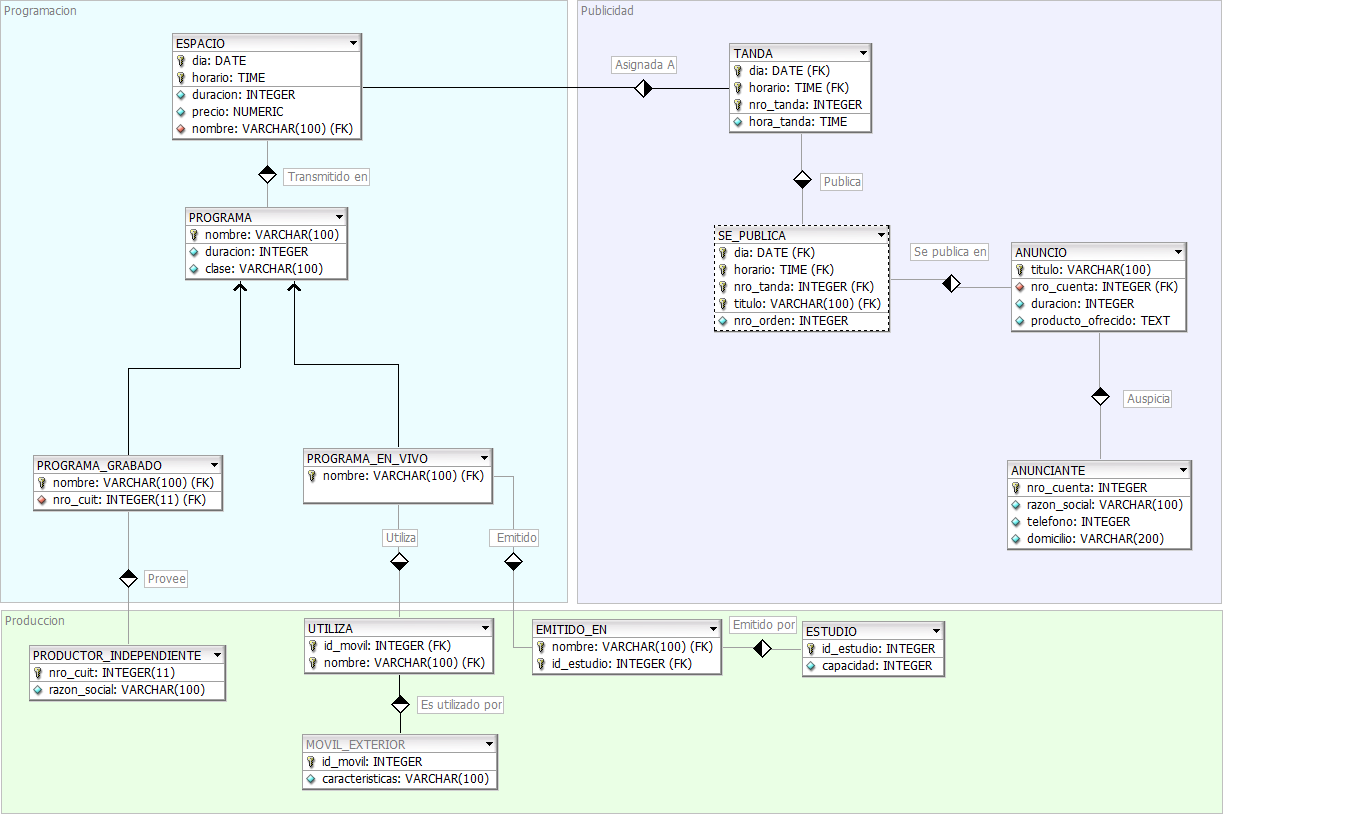
\includegraphics[scale=0.35]{der.png}
				\caption{Diagrama de modelos de tabla}
				\label{fig:flujos}
			\end{center}
		\end{figure}
		
		\begin{flushleft}
    	Algunas alternativas al diagrama presentado que se podr\'ian plantear son:
    \end{flushleft}  
    
    \begin{itemize}
    	\item Para las relaciones cuya cardinalidad \textbf{no} es N:N (ejemplo 1:N), se podr�a utilizar una tabla (como en el caso del N:N) esto tiene sus ventajas y desventajas respecto al modelo planteado. La ventaja es que resolver el problema as\'i posibilita llegado el caso cambiar la cardinalidad de la relaci�n a N:N sin mayores complicaciones. La desventaja es que esta configuraci\'on requiere una tabla m\'as y todo el esfuerzo que implica mantener esa tabla.
    	\item Para el caso particular del atributo Clase en la relaci\'on PROGRAMA, se podr\'ia usar una tabla que tenga como atributos la clase y un c\'odigo \'unico que la identifique y que almacene las diferentes clases de programas. Finalmente a la tabla PROGRAMA se la relaciona con la tabla CLASE por medio del atributo \textit{codigoclase} que se agregar\'ia en la tabla PROGRAMA (ser\'ia una clave for\'anea).
    	Se elegi\'o esta soluci\'on para mantener la simplicidad del modelo de entidad-relaci\'on.
    \end{itemize}
    
%APENDICES
\appendix
\newpage
\section{Enunciado}
  
\includepdf[pages=1-2, scale=0.8, pagecommand={\thispagestyle{plain}}]{EnunciadoBD.pdf}

\end{document}
